\tikzset{every picture/.style={line width=0.75pt}} %set default line width to 0.75pt        

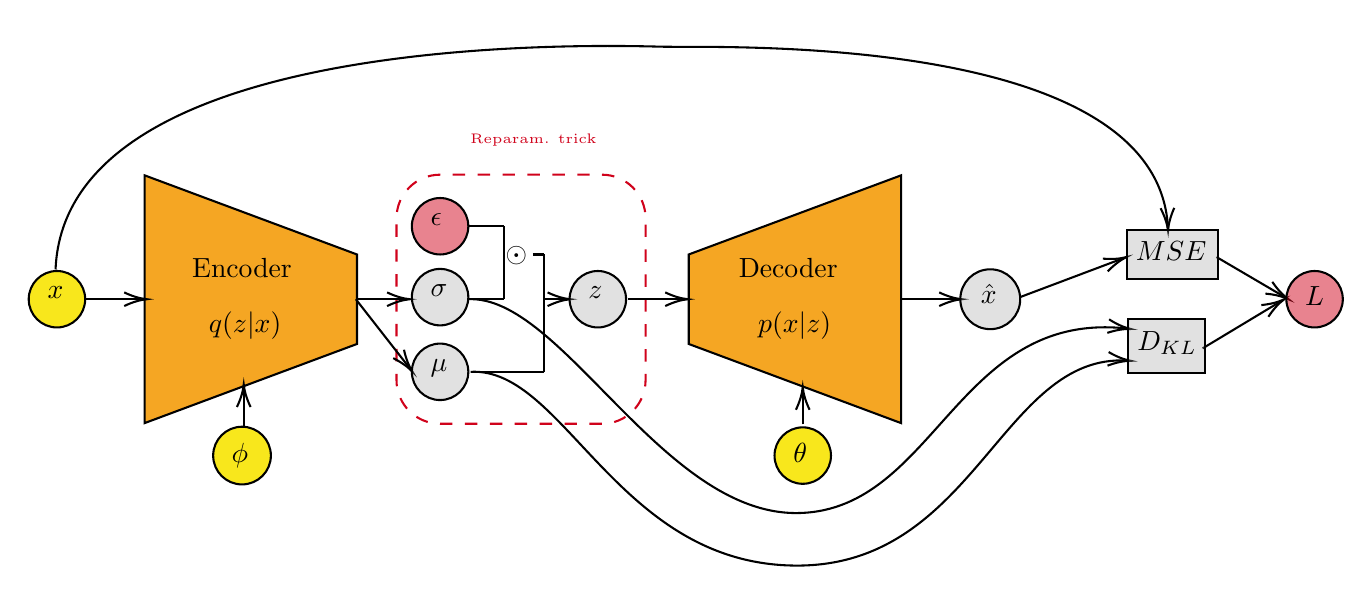
\begin{tikzpicture}[x=0.75pt,y=0.75pt,yscale=-1,xscale=1]
%uncomment if require: \path (0,300); %set diagram left start at 0, and has height of 300

%Shape: Trapezoid [id:dp7823603828525814] 
\draw  [fill={rgb, 255:red, 245; green, 166; blue, 35 }  ,fill opacity=1 ] (93.26,100.32) -- (195.56,138.44) -- (195.56,181.56) -- (93.26,219.68) -- cycle ;
%Flowchart: Alternative Process [id:dp7916519671015572] 
\draw  [color={rgb, 255:red, 208; green, 2; blue, 27 }  ,draw opacity=1 ][dash pattern={on 4.5pt off 4.5pt}] (313.6,100) .. controls (325.2,100) and (334.6,109.4) .. (334.6,121) -- (334.6,199) .. controls (334.6,210.6) and (325.2,220) .. (313.6,220) -- (235.6,220) .. controls (224,220) and (214.6,210.6) .. (214.6,199) -- (214.6,121) .. controls (214.6,109.4) and (224,100) .. (235.6,100) -- cycle ;
%Shape: Trapezoid [id:dp7878502215303758] 
\draw  [fill={rgb, 255:red, 245; green, 166; blue, 35 }  ,fill opacity=1 ] (457.69,219.68) -- (355.39,181.56) -- (355.39,138.44) -- (457.69,100.32) -- cycle ;
%Straight Lines [id:da7022493612643106] 
\draw    (65,160) -- (92.33,160) ;
\draw [shift={(94.33,160)}, rotate = 180] [color={rgb, 255:red, 0; green, 0; blue, 0 }  ][line width=0.75]    (10.93,-3.29) .. controls (6.95,-1.4) and (3.31,-0.3) .. (0,0) .. controls (3.31,0.3) and (6.95,1.4) .. (10.93,3.29)   ;
%Straight Lines [id:da842524726150703] 
\draw    (141,221.67) -- (141,203) ;
\draw [shift={(141,201)}, rotate = 90] [color={rgb, 255:red, 0; green, 0; blue, 0 }  ][line width=0.75]    (10.93,-3.29) .. controls (6.95,-1.4) and (3.31,-0.3) .. (0,0) .. controls (3.31,0.3) and (6.95,1.4) .. (10.93,3.29)   ;
%Straight Lines [id:da6004403121374124] 
\draw    (457.67,160) -- (485,160) ;
\draw [shift={(487,160)}, rotate = 180] [color={rgb, 255:red, 0; green, 0; blue, 0 }  ][line width=0.75]    (10.93,-3.29) .. controls (6.95,-1.4) and (3.31,-0.3) .. (0,0) .. controls (3.31,0.3) and (6.95,1.4) .. (10.93,3.29)   ;
%Straight Lines [id:da6888855782255758] 
\draw    (410.33,220.33) -- (410.33,204.33) ;
\draw [shift={(410.33,202.33)}, rotate = 90] [color={rgb, 255:red, 0; green, 0; blue, 0 }  ][line width=0.75]    (10.93,-3.29) .. controls (6.95,-1.4) and (3.31,-0.3) .. (0,0) .. controls (3.31,0.3) and (6.95,1.4) .. (10.93,3.29)   ;
%Straight Lines [id:da5580691014824746] 
\draw    (249.67,124.84) -- (266.6,124.84) ;
%Straight Lines [id:da0719604636131792] 
\draw    (249,160) -- (266.6,160) ;
%Straight Lines [id:da12715359384818892] 
\draw    (266.6,124.84) -- (266.6,160) ;
%Straight Lines [id:da1128909560545941] 
\draw    (285.67,194.98) -- (250.33,194.98) ;
%Straight Lines [id:da6821248002376252] 
\draw    (285.67,138.44) -- (285.67,194.98) ;
%Straight Lines [id:da18808034763917325] 
\draw    (280.33,138.44) -- (285.67,138.44) ;
%Straight Lines [id:da9818051915598998] 
\draw    (285.67,160) -- (296.33,160) ;
\draw [shift={(298.33,160)}, rotate = 180] [color={rgb, 255:red, 0; green, 0; blue, 0 }  ][line width=0.75]    (10.93,-3.29) .. controls (6.95,-1.4) and (3.31,-0.3) .. (0,0) .. controls (3.31,0.3) and (6.95,1.4) .. (10.93,3.29)   ;
%Straight Lines [id:da15034327030618333] 
\draw    (326.33,160) -- (353,160) ;
\draw [shift={(355,160)}, rotate = 180] [color={rgb, 255:red, 0; green, 0; blue, 0 }  ][line width=0.75]    (10.93,-3.29) .. controls (6.95,-1.4) and (3.31,-0.3) .. (0,0) .. controls (3.31,0.3) and (6.95,1.4) .. (10.93,3.29)   ;
%Straight Lines [id:da5118381101450515] 
\draw    (195,160) -- (219,160) ;
\draw [shift={(221,160)}, rotate = 180] [color={rgb, 255:red, 0; green, 0; blue, 0 }  ][line width=0.75]    (10.93,-3.29) .. controls (6.95,-1.4) and (3.31,-0.3) .. (0,0) .. controls (3.31,0.3) and (6.95,1.4) .. (10.93,3.29)   ;
%Straight Lines [id:da0008605514980692952] 
\draw    (195,160) -- (221.1,193.4) ;
\draw [shift={(222.33,194.98)}, rotate = 232] [color={rgb, 255:red, 0; green, 0; blue, 0 }  ][line width=0.75]    (10.93,-3.29) .. controls (6.95,-1.4) and (3.31,-0.3) .. (0,0) .. controls (3.31,0.3) and (6.95,1.4) .. (10.93,3.29)   ;
%Curve Lines [id:da606983672133339] 
\draw    (249,160) .. controls (294.33,157.67) and (343,265) .. (409,263) .. controls (474.67,261.01) and (484.9,164.64) .. (567.09,174.18) ;
\draw [shift={(568.33,174.33)}, rotate = 187.29] [color={rgb, 255:red, 0; green, 0; blue, 0 }  ][line width=0.75]    (10.93,-3.29) .. controls (6.95,-1.4) and (3.31,-0.3) .. (0,0) .. controls (3.31,0.3) and (6.95,1.4) .. (10.93,3.29)   ;
%Curve Lines [id:da10450467264141716] 
\draw    (250.33,194.98) .. controls (295.67,192.65) and (321,288.33) .. (407.67,288.33) .. controls (493.47,288.33) and (506.09,186.4) .. (566.49,189.54) ;
\draw [shift={(568.33,189.67)}, rotate = 184.92] [color={rgb, 255:red, 0; green, 0; blue, 0 }  ][line width=0.75]    (10.93,-3.29) .. controls (6.95,-1.4) and (3.31,-0.3) .. (0,0) .. controls (3.31,0.3) and (6.95,1.4) .. (10.93,3.29)   ;
%Curve Lines [id:da10659071061601377] 
\draw    (50.33,145.67) .. controls (55,29.67) and (314.33,37.67) .. (342.33,38.33) .. controls (370.19,39) and (581.54,31.08) .. (586.28,125.57) ;
\draw [shift={(586.33,127)}, rotate = 268.41] [color={rgb, 255:red, 0; green, 0; blue, 0 }  ][line width=0.75]    (10.93,-3.29) .. controls (6.95,-1.4) and (3.31,-0.3) .. (0,0) .. controls (3.31,0.3) and (6.95,1.4) .. (10.93,3.29)   ;
%Straight Lines [id:da6109248809176173] 
\draw    (515,159) -- (564.46,140.37) ;
\draw [shift={(566.33,139.67)}, rotate = 159.36] [color={rgb, 255:red, 0; green, 0; blue, 0 }  ][line width=0.75]    (10.93,-3.29) .. controls (6.95,-1.4) and (3.31,-0.3) .. (0,0) .. controls (3.31,0.3) and (6.95,1.4) .. (10.93,3.29)   ;
%Straight Lines [id:da2945225342159614] 
\draw    (609.67,139.67) -- (642.61,158.99) ;
\draw [shift={(644.33,160)}, rotate = 210.39] [color={rgb, 255:red, 0; green, 0; blue, 0 }  ][line width=0.75]    (10.93,-3.29) .. controls (6.95,-1.4) and (3.31,-0.3) .. (0,0) .. controls (3.31,0.3) and (6.95,1.4) .. (10.93,3.29)   ;
%Straight Lines [id:da8512352195616399] 
\draw    (603,183.67) -- (640.62,161.03) ;
\draw [shift={(642.33,160)}, rotate = 148.96] [color={rgb, 255:red, 0; green, 0; blue, 0 }  ][line width=0.75]    (10.93,-3.29) .. controls (6.95,-1.4) and (3.31,-0.3) .. (0,0) .. controls (3.31,0.3) and (6.95,1.4) .. (10.93,3.29)   ;

% Text Node
\draw  [fill={rgb, 255:red, 248; green, 231; blue, 28 }  ,fill opacity=1 ]  (51, 160) circle [x radius= 13.6, y radius= 13.6]   ;
\draw (45,152.4) node [anchor=north west][inner sep=0.75pt]    {$x$};
% Text Node
\draw (114.67,139) node [anchor=north west][inner sep=0.75pt]   [align=left] {Encoder};
% Text Node
\draw (122.67,164.4) node [anchor=north west][inner sep=0.75pt]    {$q( z|x)$};
% Text Node
\draw (378,139) node [anchor=north west][inner sep=0.75pt]   [align=left] {Decoder};
% Text Node
\draw (387.33,164.4) node [anchor=north west][inner sep=0.75pt]    {$p( x|z)$};
% Text Node
\draw  [fill={rgb, 255:red, 155; green, 155; blue, 155 }  ,fill opacity=0.3 ]  (500.67, 160) circle [x radius= 14.42, y radius= 14.42]   ;
\draw (494.67,151.4) node [anchor=north west][inner sep=0.75pt]    {$\hat{x}$};
% Text Node
\draw  [fill={rgb, 255:red, 248; green, 231; blue, 28 }  ,fill opacity=1 ]  (140.17, 235.33) circle [x radius= 13.9, y radius= 13.9]   ;
\draw (133.67,227.73) node [anchor=north west][inner sep=0.75pt]    {$\phi $};
% Text Node
\draw  [fill={rgb, 255:red, 208; green, 2; blue, 27 }  ,fill opacity=0.49 ]  (235.6, 124.84) circle [x radius= 13.6, y radius= 13.6]   ;
\draw (229.6,117.24) node [anchor=north west][inner sep=0.75pt]    {$\epsilon $};
% Text Node
\draw  [fill={rgb, 255:red, 248; green, 231; blue, 28 }  ,fill opacity=1 ]  (410.33, 235.33) circle [x radius= 13.6, y radius= 13.6]   ;
\draw (404.33,227.73) node [anchor=north west][inner sep=0.75pt]    {$\theta $};
% Text Node
\draw  [fill={rgb, 255:red, 155; green, 155; blue, 155 }  ,fill opacity=0.3 ]  (235.6, 159) circle [x radius= 13.6, y radius= 13.6]   ;
\draw (229.6,151.4) node [anchor=north west][inner sep=0.75pt]    {$\sigma $};
% Text Node
\draw  [fill={rgb, 255:red, 155; green, 155; blue, 155 }  ,fill opacity=0.3 ]  (235.6, 194.98) circle [x radius= 13.6, y radius= 13.6]   ;
\draw (229.6,187.38) node [anchor=north west][inner sep=0.75pt]    {$\mu $};
% Text Node
\draw  [fill={rgb, 255:red, 155; green, 155; blue, 155 }  ,fill opacity=0.3 ]  (311.6, 160) circle [x radius= 13.6, y radius= 13.6]   ;
\draw (305.6,152.4) node [anchor=north west][inner sep=0.75pt]    {$z$};
% Text Node
\draw (265.67,132.84) node [anchor=north west][inner sep=0.75pt]    {$\odot $};
% Text Node
\draw  [fill={rgb, 255:red, 155; green, 155; blue, 155 }  ,fill opacity=0.3 ]  (566.33,126.44) -- (610.33,126.44) -- (610.33,150.44) -- (566.33,150.44) -- cycle  ;
\draw (569.33,130.84) node [anchor=north west][inner sep=0.75pt]    {$MSE$};
% Text Node
\draw  [fill={rgb, 255:red, 155; green, 155; blue, 155 }  ,fill opacity=0.3 ]  (567,169.56) -- (604,169.56) -- (604,195.56) -- (567,195.56) -- cycle  ;
\draw (570,173.96) node [anchor=north west][inner sep=0.75pt]    {$D_{KL}$};
% Text Node
\draw (248.67,79) node [anchor=north west][inner sep=0.75pt]  [color={rgb, 255:red, 208; green, 2; blue, 27 }  ,opacity=1 ] [align=left] {{\tiny Reparam. trick}};
% Text Node
\draw  [fill={rgb, 255:red, 208; green, 2; blue, 27 }  ,fill opacity=0.49 ]  (656.93, 160) circle [x radius= 13.6, y radius= 13.6]   ;
\draw (650.93,152.4) node [anchor=north west][inner sep=0.75pt]    {$L$};


\end{tikzpicture}